\section{Introduction}

%Bayesian analysis is a cornerstone of modern statistical inference. It uses Bayes theorem to iteratively update the probability of a given hypothesis or model (posterior) given existing knowledge about the model parameters (prior) and a representative probability distribution for the data given the choice of model and parameters at each iteration (likelihood). Various computational approaches to Bayesian analysis exist, including Markov Chain Monte Carlo~(MCMC) methods \citep[e.g.][]{emcee} and Nested Sampling algorithms \citep[e.g.][]{polychord_2015, polychord_2015b}.

Bayesian analysis has been applied in the inference of cosmological parameters from experiments such as the CMB mapper Planck~\cite{Planck2018}, the Dark Energy Survey~(DES, \citep{DES_Year1_2018, DES_year3_2021, DES_year3}), 21-cm power spectrum experiments~(such as HERA~\citep{HERA_2022b}, LOFAR~\citep{Ghara_LOFAR_2020, Mondal_LOFAR_2020} and MWA~\citep{Greig_MWA_2020, Ghara_MWA_2021}) and global or sky-averaged 21-cm experiments such as
REACH~\citep{Anstey_REACH_2021} and SARAS \citep{Bevins_SARAS2_2022, Bevins_saras3_2022}. 

These experiments are often plagued by `nuisance' parameters that characterise foregrounds and instrumental effects in the data. This leads to high dimensional parameter spaces, of which only a few of the parameters model the core science. Consequently, drawing conclusions about the parameters of interest and making comparisons of different experiments can be challenging. For example, in the Year 1 analysis of data from DES the likelihood contains a total of 26 parameters of which 20 could be considered nuisance parameters with only 6 corresponding to cosmological parameters of interest~\citep{DES_Year1_2018}. Similarly, for REACH \citep{Anstey_REACH_2021, de_lera_acedo_reach_2022} the likelihood can contain around 20–30 parameters, with only 3-7 of these corresponding to the signal.

In this chapter, we present a post-processing tool called \textsc{margarine} that can be used to calculate \emph{marginal} or \emph{nuisance-free} posterior distributions pertaining to the core science goals of the above experiments through density estimation with Masked Autoregressive Flows~(MAFs, \cite{Papamarkarios_MAF_2017}) and Kernel Density Estimators~(KDEs, \cite{rosenblatt_KDE_1956, parzen_KDE_1962}).

Due to the ubiquity of Bayesian analysis in cosmology, post-processing of samples from MCMC and Nested Sampling algorithms is an important area of research. \textsc{margarine} is an invaluable addition to the Bayesian workflow and allows for direct and specific comparison of the constraining ability of different experimental approaches, rapid emulation of nuisance-free likelihoods and experimentally informed priors.

We implement our approach in \textsc{Python} using \textsc{tensorflow} and the \textsc{keras} backend and release the code as the pip installable package \textsc{margarine}. The code is fully documented with worked examples, subject to continuous integration testing and does not require high performance computing to be used.

In \cref{sec:motivation}, we briefly outline the motivation behind the development of \textsc{margarine}. In \cref{sec:theory}, we reintroduce Bayesian analysis and discuss the marginal statistical quantities that can be calculated with \textsc{margarine}. We discuss the two different types of density estimators used by \textsc{margarine} in \cref{sec:density_estimators}. In \cref{sec:applications}, we demonstrate several applications of the code base, including applications to samples from the Dark Energy Survey, Planck and mock observations with the REACH pipeline. We summarise the chapter in \cref{sec:conclusions_margarine}.

%\textsc{margarine} was previously introduced in the conference proceedings for the 2022 International Conference on Bayesian and Maximum Entropy Methods in Science and Engineering \citep[MaxEnt22, ][]{margarine_maxent} in which the nuisance-free likelihood was derived and demonstrated. We review this work briefly in this chapter.

\Cref{sec:marginal_likelihood} was first drafted by Will Handley for \cite{margarine_maxent}, edited by the author and visualized in \cref{fig:pipeline} and \cref{fig:pipelineB} by the author. The co-authors, Will Handley, Pablo Lemos, Peter Sims, Eloy de Lera Acedo, Anastasia Fialkov and Justin Alsing, of \cite{margarine_maxent} and \cite{margarine_neurips} provided comments on the manuscripts that this chapter is adapted from.

\section{Motivation}
\label{sec:motivation}

If our model $M (\Theta)$ contains nuisance, $\alpha$, and cosmological signal parameters, $\theta$, then we can write $\Theta = \{\alpha, \theta\}$. Mathematically, the marginal posterior for the signal parameters, $\mathcal{P}(\theta)$, can be calculated by integrating out the dependence on $\alpha$
\begin{equation}
    \mathcal{P}(\theta) = \int \mathcal{P}(\alpha, \theta) d \alpha.
    \label{eq:marginal_posterior}
\end{equation}
However, $\mathcal{P}(\theta)$ is typically a difficult quantity to calculate. We can effectively perform this marginalisation by training density estimators on samples in $\theta$ from MCMC or Nested Sampling chains. From these density estimators, we can generate samples from the marginal distribution $\mathcal{P}(\theta)$ and importantly calculate $\log \mathcal{P}(\theta)$ for a given set of $\theta$, which gives us access to a whole host of previously intractable marginal summary statistics.

For example, the marginal Kullback-Leibler~(KL) divergence tells you how much information is gained by contracting specifically the core science prior onto the core science posterior without including contributions from correlations with or constraints on the nuisance parameters. This allows us to confidently compare the information gained from different data sets from different experiments measuring the same signal, regardless of their specific instrumental nuances. Similarly, the marginal Bayesian Model Dimensionality~(BMD) can be used to compare the effective number of core science parameters constrained by different experiments and models. Both the \emph{marginal} KL divergence and the BMD, therefore, provide a way to quantitatively determine which experimental approaches are the most informative, which can inform improvements to instrumentation in the future and prior to \textsc{margarine} was not as easy to assess.

Using normalised density estimators to calculate the KL divergence, marginal or not, also has the added advantage that it does not require knowledge of the Bayesian evidence, which is not always accessible.

Further, since the density estimators can be used to empirically approximate the logarithm of any posterior distribution, then they can be used as a computationally inexpensive likelihood generator. In practice, we can take advantage of this to perform efficient analysis of constraints from multiple different experiments as demonstrated in this chapter and further in \cref{ch:hera_saras3}.

Finally, we note that if the density estimator is set up correctly such that it is a bijective transformation between the unit hyper-cube and the target posterior, then it can be used to generate the prior on a subsequent Nested Sampling run. This allows you to use far more complex priors based on current experimental results, incorporating our current knowledge of the parameter space~\citep{Alsing_bijectors_2021}.

\section{Theory}
\label{sec:theory}

\subsection{Bayesian analysis}
\label{sec:bayesian_inference}

Bayesian analysis is concerned with the estimation of posterior probabilities using Bayes theorem
\begin{equation}
    P(\Theta | D, M) = \frac{P(D| \Theta, M) P(\Theta|M)}{P(D|M)} = \frac{\mathcal{L}(\Theta)\pi(\Theta)}{\mathcal{Z}},
    \label{eq:bayes_theorem}
\end{equation}
where $\Theta$ are the parameters of our model $M$ describing the data $D$ and $\mathcal{L}(\Theta)$ corresponds to the likelihood. The likelihood is often assumed to be Gaussian in nature (although more complicated likelihoods can be implemented~\cite{Scheutwinkel2022a}). The prior, $\pi(\Theta) = P(\Theta|M)$, encodes our existing knowledge about the parameters before any sampling is performed. $\pi(\Theta)$ is often chosen to be uniform or log-uniform for each parameter, however we would often like to inform this with existing experimental results.

The evidence, $\mathcal{Z}$, is a (fully-)marginal likelihood integrated over all the parameters and weighted by the prior
\begin{equation}
    \mathcal{Z} = \int \mathcal{L}(\Theta)\pi(\Theta)d\Theta.
    \label{eq:evidence}
\end{equation}

\subsection{Nuisance-free likelihood}
\label{sec:marginal_likelihood}

We can re-write Bayes theorem as
\begin{equation}
     \mathcal{L}(\theta,\alpha)\times \pi(\theta,\alpha) =\mathcal{P}(\theta,\alpha)\times \mathcal{Z},
    \label{eqn:bayes}
\end{equation}
with the inputs of inference (likelihood and prior) on the left-hand side, and the outputs (posterior and evidence) on the right.

We may marginalise any probability distribution so can, in addition to the definition of the nuisance marginalised posterior, straightforwardly define the nuisance marginalised prior by integrating over $\alpha$
\begin{equation}
    \pi(\theta) = \int \pi(\theta,\alpha)d\alpha.
    \label{eqn:marginal}
\end{equation}
The nuisance marginalised version of Bayes theorem~\cref{eqn:bayes} takes the form
\begin{equation}
    \mathcal{L}(\theta)\times\pi(\theta) = \mathcal{P}(\theta)\times\mathcal{Z}.
    \label{eqn:marginal_bayes}
\end{equation}
Here $\mathcal{Z}$ is the original evidence, whilst $\mathcal{L}(\theta)$ is non-trivially the \emph{nuisance-free likelihood}
\begin{equation}
    \mathcal{L}(\theta) 
\equiv \frac{\int\mathcal{L}(\theta,\alpha)\pi(\theta,\alpha)d\alpha}{\int \pi(\theta,\alpha)d\alpha} = \frac{\mathcal{P}(\theta)\mathcal{Z}}{\pi(\theta)},
    \label{eqn:partial}
\end{equation}
where the above is motivated by marginalising Bayes theorem over $\alpha$, and substituting the definitions in \cref{eqn:partial,eq:marginal_posterior,eqn:marginal} recovers the marginalised Bayes theorem~\cref{eqn:marginal_bayes}.

The nuisance-free likelihood \cref{eqn:partial} is straightforward to compute in our framework since we (uniquely) have Nested Sampling-computed evidences $\mathcal{Z}$ and we can generate emulators for the distributions $\mathcal{P}(\theta)$ and $\pi(\theta)$ with \textsc{margarine}.

Let $\mathcal{L}_A(\theta,\alpha_A)$ and $\mathcal{L}_B(\theta,\alpha_B)$ be two likelihoods for distinct datasets, each with their own nuisance parameters. The nuisance-free likelihoods $\mathcal{L}_A(\theta)$, $\mathcal{L}_B(\theta)$ form a lossless compression in $\theta$. This means that we can recover the same (marginal) inference in combination that we would have made when performing a combined analysis with all nuisance parameters:
\begin{align}
    \mathcal{L}_A(\theta,\alpha_A)\mathcal{L}_B(\theta,\alpha_B)\pi_{AB}(\theta,\alpha_A,\alpha_B) &=  \mathcal{P}_{AB}(\theta,\alpha_A,\alpha_B)\mathcal{Z}_{AB},  \label{eqn:combined_bayes}\\
    \Rightarrow
        \mathcal{L}_A(\theta)\mathcal{L}_B(\theta)\pi(\theta) &=  \mathcal{P}_{AB}(\theta)\mathcal{Z}_{AB}, 
        \label{eqn:marginal_combined_bayes}
\end{align}
 if their respective priors $\pi_A(\theta,\alpha_A)$ and $\pi_B(\theta,\alpha_B)$ satisfy the marginal consistency relations:
\begin{gather}
    \pi(\theta) = \int \pi_A(\theta,\alpha_A)d\alpha_A = \int \pi_B(\theta,\alpha_B)d\alpha_B,  
    \label{eqn:marginal_A}\\
    \int \pi_{AB}(\theta,\alpha_A,\alpha_B)d\alpha_A = \pi_B(\theta,\alpha_B), \qquad \int \pi_{AB}(\theta,\alpha_A,\alpha_B)d\alpha_B = \pi_A(\theta,\alpha_A).
    \label{eqn:marginal_B}
\end{gather}
This process is represented graphically in \cref{fig:pipeline} and \cref{fig:pipelineB}.

\begin{figure}
\centering
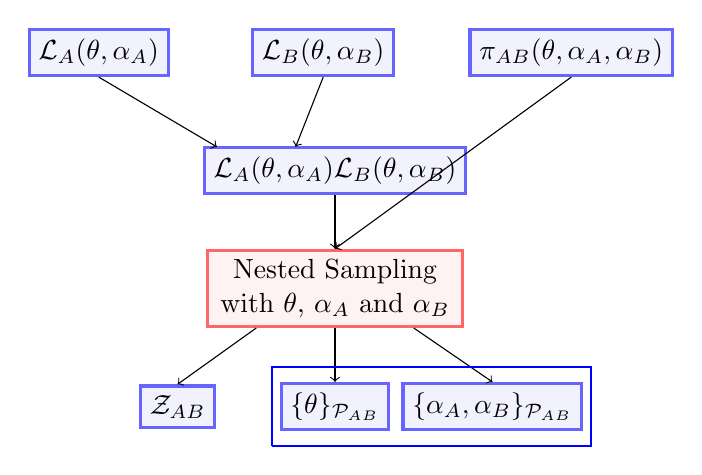
\begin{tikzpicture}[squarednodeA/.style={rectangle, draw=red!60, fill=red!5, very thick, minimum size=5mm},
squarednodeB/.style={rectangle, draw=blue!60, fill=blue!5, very thick, minimum size=5mm},
squarednodeC/.style={rectangle, draw=green!60, fill=green!5, very thick, minimum size=5mm}]

\node[squarednodeA, text width=3cm, align=center](inference3) at (17, -1.5) {Nested Sampling with $\theta$, $\alpha_A$ and $\alpha_B$};

\node[squarednodeB](fulllikelihood1) at (14, 1.5){$ \mathcal{L}_A(\theta,\alpha_A)$};
\node[squarednodeB](fulllikelihood2) at (16.85, 1.5){$ \mathcal{L}_B(\theta,\alpha_B)$};
\node[squarednodeB](fulljointlikelihood) at (17, 0){$ \mathcal{L}_A(\theta,\alpha_A) \mathcal{L}_B(\theta,\alpha_B)$};
\node[squarednodeB](fullprior) at (20, 1.5){$ \pi_{AB}(\theta,\alpha_A, \alpha_B)$};

\draw[->](fulllikelihood1.south) -- (15.5, 0.3);
\draw[->](fulllikelihood2.south) -- (16.5, 0.3);
\draw[->](fullprior.south) -- (inference3.north);
\draw[->](fulljointlikelihood.south) -- (inference3.north);

\node[squarednodeB](jointEvidence2) at (15, -3){$ \mathcal{Z}_{AB}$};
\node[squarednodeB](jointPosterior2) at (17, -3){$ \{\theta\}_{\mathcal{P}_{AB}}$};

\draw[<-](jointEvidence2.north) -- (16, -2);
\draw[<-](jointPosterior2.north) -- (inference3.south);

\node[squarednodeB](jointPosteriorNuisance) at (19, -3){$ \{\alpha_A, \alpha_B\}_{\mathcal{P}_{AB}}$};
\draw[->](18, -2) -- (jointPosteriorNuisance.north);
\draw[blue,thick](16.2, -3.5) -- (20.25, -3.5) -- (20.25, -2.5) -- (16.2, -2.5) -- (16.2, -3.5);

\end{tikzpicture}
\caption{A graphical representation of combining constraints from different data sets via a full Nested Sampling run over both cosmological and nuisance parameters (\cref{eqn:combined_bayes}).}
\label{fig:pipeline}
\end{figure}

\begin{figure}
\centering
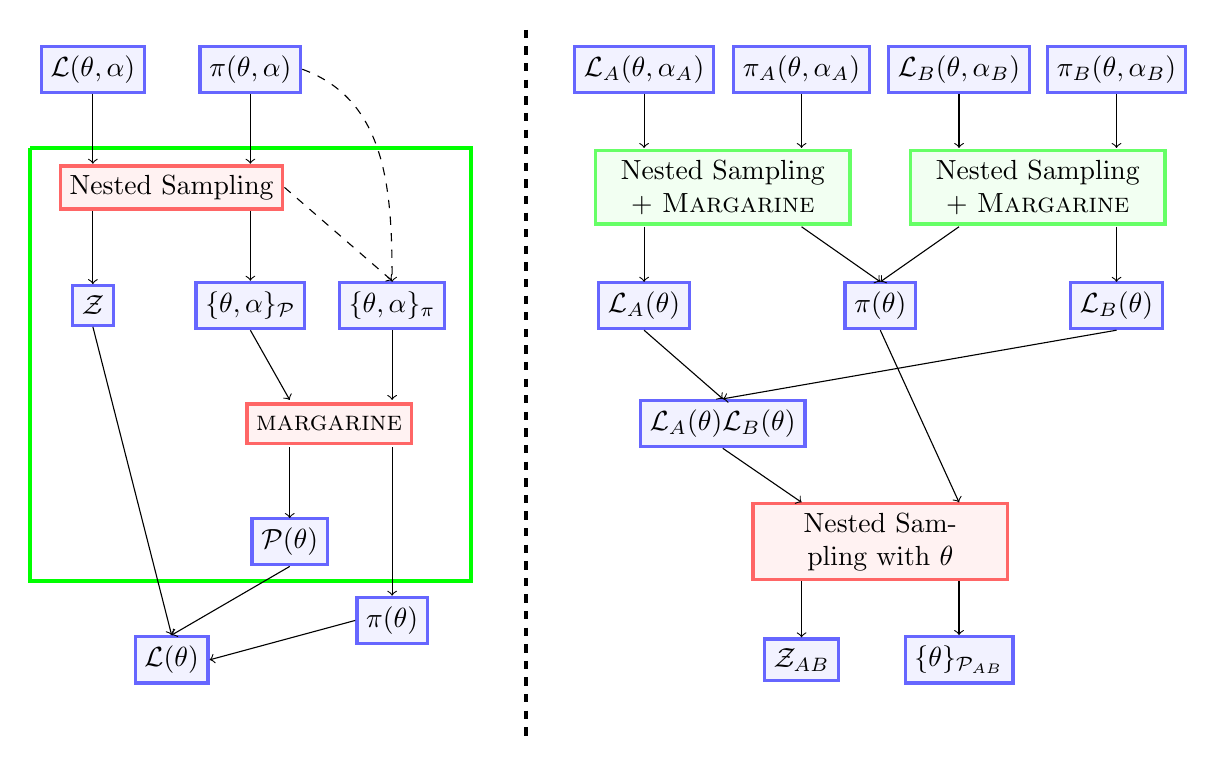
\begin{tikzpicture}[squarednodeA/.style={rectangle, draw=red!60, fill=red!5, very thick, minimum size=5mm},
squarednodeB/.style={rectangle, draw=blue!60, fill=blue!5, very thick, minimum size=5mm},
squarednodeC/.style={rectangle, draw=green!60, fill=green!5, very thick, minimum size=5mm}]
\node[squarednodeA](inference) at (0, 0) {Nested Sampling};
\node[squarednodeB](likelihood) at (-1, 1.5){$ \mathcal{L}(\theta,\alpha)$};
\node[squarednodeB](prior) at (1, 1.5){$ \pi(\theta,\alpha)$};
\node[squarednodeB](evidence) at (-1, -1.5){$ \mathcal{Z}$};
\node[squarednodeB](posterior) at (1, -1.5){$ \{\theta,\alpha\}_\mathcal{P}$};
\node[squarednodeB](priorSamples) at (2.8, -1.5){$ \{\theta,\alpha\}_\pi$};
\node[squarednodeA](margarine) at (2, -3) {\textsc{margarine}};
\node[squarednodeB](marginalPrior) at (2.8, -5.5){$ \pi(\theta)$};
\node[squarednodeB](marginalPosterior) at (1.5, -4.5){$ \mathcal{P}(\theta)$};
\node[squarednodeB](marginalLikelihood) at (0, -6){$ \mathcal{L}(\theta)$};

\draw[green, ultra thick] (-1.8, 0.5) -- (-1.8, -5) -- (3.8, -5)-- (3.8, 0.5) -- (-1.8, 0.5);

\draw[->](likelihood.south) -- (-1, 0.3);
\draw[->](prior.south) -- (1, 0.3);
\draw[->](-1, -0.3) -- (evidence.north);
\draw[->](1, -0.3) -- (posterior.north);
\draw[->](posterior.south) -- (1.5, -2.7);
\draw[dashed,->](prior.east) to[out=-20, in=90] (2.8, -1.2);
\draw[->](priorSamples.south) -- (2.8, -2.7);
\draw[->](2.8, -3.3) -- (marginalPrior.north);
\draw[->](1.5, -3.3) -- (1.5, -4.2);
\draw[->](evidence.south) -- (marginalLikelihood.north);
\draw[->](marginalPosterior.south) -- (marginalLikelihood.north);
\draw[->](marginalPrior.west) -- (marginalLikelihood.east);
\draw[dashed,->](inference.east) -- (priorSamples.north);

\draw[black, ultra thick, dashed] (4.5, 2) -- (4.5, -7);

\node[squarednodeB](likelihood1) at (6, 1.5){$ \mathcal{L}_A(\theta,\alpha_A)$};
\node[squarednodeB](prior1) at (8, 1.5){$ \pi_A(\theta,\alpha_A)$};

\node[squarednodeC, text width=3cm, align=center](NestedMarg1) at (7, 0){Nested Sampling + \textsc{Margarine}};

\draw[->](likelihood1.south) -- (6, 0.5);
\draw[->](prior1.south) -- (8, 0.5);

\node[squarednodeB](marglike1) at (6, -1.5){$ \mathcal{L}_A(\theta)$};
\node[squarednodeB](margprior1) at (9, -1.5){$ \pi(\theta)$};

\draw[->](6, -0.5) -- (6, -1.2);
\draw[->](8, -0.5) -- (9, -1.2);

\node[squarednodeB](likelihood2) at (10, 1.5){$ \mathcal{L}_B(\theta,\alpha_B)$};
\node[squarednodeB](prior2) at (12, 1.5){$ \pi_B(\theta,\alpha_B)$};

\draw[->](likelihood2.south) -- (10, 0.5);
\draw[->](prior2.south) -- (12, 0.5);

\node[squarednodeC, text width=3cm, align=center](NestedMarg1) at (11, 0){Nested Sampling + \textsc{Margarine}};

\node[squarednodeB](marglike2) at (12, -1.5){$ \mathcal{L}_B(\theta)$};
\draw[->](12, -0.5) -- (12, -1.2);
\draw[->](10, -0.5) -- (9, -1.2);

\node[squarednodeB](combinedlike) at (7, -3){$ \mathcal{L}_A(\theta) \mathcal{L}_B(\theta)$};

\draw[->](marglike1.south) -- (combinedlike.north);
\draw[->](marglike2.south) -- (combinedlike.north);

\node[squarednodeA, text width=3cm, align=center](inference2) at (9, -4.5) {Nested Sampling with $\theta$};

\draw[->](combinedlike.south) -- (8, -4);
\draw[->](margprior1.south) -- (10, -4);

\node[squarednodeB](jointEvidence) at (8, -6){$ \mathcal{Z}_{AB}$};
\node[squarednodeB](jointPosterior) at (10, -6){$ \{\theta\}_{\mathcal{P}_{AB}}$};

\draw[->](8, -5) -- (jointEvidence.north);
\draw[->](10, -5) -- (jointPosterior.north);

%%%%%%%%%%%%%%%%%%%%%%%%%%%%%%%%%%%%%%%%%%%%%%%%%%%%%%%%%%%%%%%%%%%%%%%

\end{tikzpicture}
\caption{A graphical representation of combining constraints from two data sets via \textsc{margarine} (\cref{eqn:marginal_combined_bayes}). Left of the dashed line illustrates the derivation of a nuisance-free likelihood function for one experimental data set.}
\label{fig:pipelineB}
\end{figure}

Integrating the combined Bayes theorem \cref{eqn:combined_bayes} with respect to $\alpha_B$, applying the definition of the marginal posterior \cref{eqn:marginal} on the right-hand side, and drawing out terms independent of $\alpha_B$ on the left,  yields
\begin{equation}
    \mathcal{L}_A(\theta,\alpha_A)\int\mathcal{L}_B(\theta,\alpha_B)\pi_{AB}(\theta,\alpha_A,\alpha_B)d\alpha_B =  \mathcal{P}_{AB}(\theta,\alpha_A)\mathcal{Z}_{AB}.
    \label{eqn:temp1}
\end{equation}
From the definition of a nuisance-free likelihood~\cref{eqn:partial}, and the marginal consistency~\cref{eqn:marginal_B}, we can say that the integral on the left-hand side becomes:
\begin{align}
    &\int \mathcal{L}_B(\theta,\alpha_B) \pi_{AB}(\theta,\alpha_A,\alpha_B)d\alpha_B \nonumber\\
    &= \int \mathcal{L}_B(\theta,\alpha_A,\alpha_B) \pi_{AB}(\theta,\alpha_A,\alpha_B)d\alpha_B 
    &\left[\text{$\mathcal{L}_B(\theta,\alpha_B)\equiv \mathcal{L}_B(\theta,\alpha_A,\alpha_B)$ since $\mathcal{L}_B$ indep of $\alpha_A$}\right]
    \nonumber\\
    &= \mathcal{L}_B(\theta,\alpha_A) {\int \pi_{AB}(\theta,\alpha_A,\alpha_B) d\alpha_B} 
    &\left[\text{Using \cref{eqn:partial} for $\mathcal{L}_B$}\right]
    \nonumber\\
    &= \mathcal{L}_B(\theta) {\int \pi_{AB}(\theta,\alpha_A,\alpha_B) d\alpha_B} 
    &\left[\text{$\mathcal{L}_B(\theta,\alpha_A)\equiv \mathcal{L}_B(\theta)$ since $\mathcal{L}_B$ indep of $\alpha_A$}\right]
    \nonumber\\
    &= \mathcal{L}_B(\theta) \pi_A(\theta,\alpha_A).
    &\left[\text{Using marginal consistency \cref{eqn:marginal_B}}\right]
    \label{eqn:temp2}
\end{align}
Substituting \cref{eqn:temp2} back into \cref{eqn:temp1} we find
\begin{equation}
    \mathcal{L}_A(\theta,\alpha_A)\mathcal{L}_B(\theta)\pi_A(\theta,\alpha_A) =  \mathcal{P}_{AB}(\theta,\alpha_A)\mathcal{Z}_{AB}.
\end{equation}
Proceeding with a similar manipulation to \cref{eqn:temp2}, marginalising with respect to $\alpha_A$, and applying the definition of the nuisance-free likelihood $\mathcal{L}_A(\theta)$ \cref{eqn:partial} and the marginal prior consistency~\cref{eqn:marginal_A} we recover \cref{eqn:marginal_combined_bayes}
\begin{equation}
    \mathcal{L}_A(\theta)\mathcal{L}_B(\theta)\pi(\theta) =  \mathcal{P}_{AB}(\theta)\mathcal{Z}_{AB}. \nonumber
\end{equation}

\Cref{eqn:combined_bayes} represents Bayes theorem for the combined likelihood of both  datasets $\mathcal{L}_{AB}(\theta,\alpha_A,\alpha_B) = \mathcal{L}_A(\theta,\alpha_A)\mathcal{L}_B(\theta,\alpha_B)$, using the combined prior $\pi_{AB}(\theta,\alpha_A,\alpha_B)$. We assume the combined prior is marginally consistent, \cref{eqn:marginal_A,eqn:marginal_B}, which is reasonable, merely demanding that the priors are identical in the parameter spaces where they overlap. In practice, this would usually be achieved by assuming separability between signal and nuisance parameter spaces $\pi(\theta,\alpha) = \pi(\theta)\pi(\alpha)$, but \cref{eqn:marginal_A,eqn:marginal_B} are a slightly less restrictive requirement and therefore more general. 

The upshot of this is that if you have performed inference for two datasets separately, such that you are able to compute the nuisance-free likelihoods with \textsc{margarine}, you may discard the nuisance parameters for the next set of analyses when you combine the datasets as in \cref{fig:pipelineB}.

We demonstrate applications of the nuisance-free likelihood in \cref{sec:nuisance_free_likelihood_apps} with a simple toy example and a real world example combining constraints on data from Planck and the Dark Energy Survey.

\subsection{Marginal Kullback-Leibler divergence}

The KL divergence quantifies the contraction from prior to posterior. The \emph{marginal} KL divergence corresponding to the astrophysical parameters $\theta$ is defined as the average Shannon Information
\begin{equation}
    \mathcal{I}(\theta) = \log\frac{\mathcal{P}(\theta)}{\pi(\theta)}
    \label{eq:shannon_entropy}
\end{equation}
over the posterior, $\mathcal{P}(\theta)$,
\begin{equation}
    \mathcal{D}(\mathcal{P}||\pi) = \int \mathcal{P}(\theta) \log\frac{\mathcal{P}(\theta)}{\pi(\theta)} d\theta = \left\langle \mathcal{I} \right\rangle_\mathcal{P} \approx \log\frac{V_\pi}{V_\mathcal{P}},
    \label{eq:kl_divergence}
\end{equation}
and is a measure of how much information in bits the data provides us about the parameter space, which we can think of as the constraining power of the data. It is approximately equal to the log of the ratio of the prior volume,$V_\pi$, and the posterior volume, $V_\mathcal{P}$. $\mathcal{D}$ is a strong function of the prior, and inherits the property of being additive for independent parameters from the Shannon Information. Calculation of the KL divergence requires the posterior distribution to be appropriately normalised and consequently the quantity is not attainable with common MCMC sampling techniques and more computationally intensive algorithms such as Nested sampling have to be implemented to attain the Bayesian evidence.

%It is also an anti-symmetric function which can be seen by decomposing \cref{eq:kl_divergence} into a cross-entropy and entropy term
%\begin{equation}
%    \mathcal{D(\mathcal{P}||\pi)} = \langle-\log(\pi)\rangle_\mathcal{P} + \langle\log(\mathcal{P})\rangle_\mathcal{P},
%\end{equation}
%which is not the same as
%\begin{equation}
%    \mathcal{D(\pi||\mathcal{P})} = \langle-\log(\mathcal{P})\rangle_\pi + \langle\log(\pi)\rangle_\pi,
%\end{equation}
%since the expectation values are taken over different probability distributions.

%A higher KL divergence indicates a larger information gain when moving from the prior to the posterior. This information gain is not always visible in the traditionally used corner plots showing 1D and 2D marginal posteriors, and consequently the KL divergence is a useful measure of the constraining power of the data~\cite{Handley_dimensionality_2019}. %An example of this is shown in Fig. 1 of~\cite{Handley_dimensionality_2019} in which we can see that a correlation in two dimensions gives the same KL divergence as a more obvious pair of tight constraints in the individual dimension.

%The KL divergence can be shown to be invariant under a change of variables, % $x \rightarrow y$ since a given probability distribution, $P(x)$, can be related to $P(y)$ via
%\begin{equation}
%    P(x) = P(y) \frac{dy}{dx}.
%\end{equation}
%meaning that its value in complex hard to learn spaces can be calculated in simpler transformed spaces (see \cref{sec:density_estimators}).

%This means that the prior and the posterior distributions can be transformed into a different parameter space to calculate the KL divergence. As long as that transformation is the same for each distribution the KL divergence will be equal to the value in the original parameter space.

\subsection{Marginal Bayesian Model Dimensionality}

An alternative measure of constraint is the Bayesian Model Dimensionality~\cite{Handley_dimensionality_2019} which gives a measure of the effective number of parameters that are being constrained and can be used to quantify tensions between different experimental results~\cite{Handley_tensions_2019,2022arXiv220505892G}.
The \emph{marginal} BMD $d$ is given by
\begin{equation}
    \begin{split}
    \frac{d}{2} &= \int \mathcal{P}(\theta) \bigg(\log\frac{\mathcal{P}(\theta)}{\pi(\theta)} - \mathcal{D}\bigg)^2 d\theta \\
    & = \mathrm{var}(\mathcal{I})_\mathcal{P} \\
    & = \langle(\log \mathcal{L})^2\rangle_\mathcal{P} - \langle\log\mathcal{L}\rangle_\mathcal{P}^2,
    \end{split}
    \label{eq:bayesian_dimensionality}
\end{equation}
and a full derivation can be found in~\cite{Handley_dimensionality_2019}. 
The quantity is the variance of the Shannon information and therefore a higher order statistic than the KL divergence.
It is only weakly prior dependent and like the KL divergence is additive for independent parameters and invariant under a change of variables.

\section{Density Estimators in Practice}
\label{sec:density_estimators}

In principle, you can use any type of density estimator to model subspaces in a larger parameter space and calculate the marginal Bayesian statistics discussed. The only requirements are that it can be used to resample the space and approximate the normalised log-probability associated with the posterior subspace.

\subsection{Masked Autoregressive Flows}

Complex densities are best estimated using expressive neural networks that have been trained to transform between some base distribution, often a standard normal, and the target probability distribution, e.g. the posterior from a Bayesian Nested Sampling run. \textsc{margarine} uses Masked Autoregressive Flows~(MAF) \cite{Papamarkarios_MAF_2017}, which are discussed extensively in the introduction of this thesis, to perform this transformation.%, and we typically use a multivariate standard normal distribution, $z_0 \sim \mathcal{N}(0, 1)$, as our base distribution.

\begin{comment}
An example Masked Autoencoder for Distribution Estimation~(MADE) neural network, which forms the basis of the MAF, is shown in \cref{fig:maf}. The network works by dividing the target probability distribution into a series of one dimensional conditional distributions
\begin{equation}
P(\theta) = \prod_i P(\theta_i| \theta_1, \theta_2, ..., \theta_{i-1}),
\label{eq:conditional_1}
\end{equation}
and modelling each conditional probability as a Gaussian
\begin{equation}
P(\theta_i| \theta_1, \theta_2, ..., \theta_{i-1}) = \sigma_i \mathcal{N}(0, 1) + \mu_i,
\label{eq:conditional_2}
\end{equation}
where $\sigma_i$ and $\mu_i$ are parameters that shift and scale the distributions. The network is not fully connected, but masked to represent the conditionality in \cref{eq:conditional_1}.

We input samples from $\theta$ into the network and output values of $\sigma$ and $\mu$ which are then used to reconstruct the standard normal distribution with
\begin{equation}
    z_i = \frac{(\theta_i - \mu_i)}{\sigma_i}.
    \label{eq:reconstruction_maf}
\end{equation}
The vectors of $\sigma$ and $\mu$ are therefore functions of the networks weights and biases that need to be trained.

We train the weights and biases using the change of variables formula
\begin{equation}
    P(x) = P(z) \bigg|\frac{\delta z}{\delta x}\bigg|,
\end{equation}
where the goal is to minimize the difference between a true standard normal distribution and the reconstructed `standard normal' corresponding to \cref{eq:reconstruction_maf}. In practice, our network loss looks like
\begin{equation}
    \mathrm{min}(-\log(P(z^\prime)) - \log(\bigg|\frac{\delta z^\prime}{\delta z}\bigg|)),
\end{equation}
and we can interpret the second term in this equation as the change in volume between the standard normal distribution and the network output $z^\prime$. If the second term is $\approx 0$ we can be confident that our network is correctly transforming samples from our posterior into samples on the standard normal.

Importantly, the MADE networks are bijective, and we can therefore, once trained, use them to transform samples on the standard normal into samples from the target posterior.

\begin{figure*}
    \centering
    \begin{tikzpicture}[rednode/.style={circle, draw=red!60, fill=red!5, very thick, minimum size=5mm},
                bluenode/.style={circle, draw=blue!60, fill=blue!5, very thick, minimum size=5mm},
                greennode/.style={circle, draw=green!60, fill=green!5, very thick, minimum size=5mm},
                node distance=0.5cm and 2cm,
                remember picture]
        \node (0) {};
        
        \node[rednode, above=of 0, text width=0.5cm, align=center](layer1_center1) {$\mu_2$};
        \node[rednode, below=of layer1_center1, text width=0.5cm, align=center](layer1_center2) {$\sigma_2$};
        \node[rednode, above=of layer1_center1, text width=0.5cm, align=center](layer1_top2) {$\sigma_1$};
        \node[rednode, above=of layer1_top2, text width=0.5cm, align=center](layer1_top1) {$\mu_1$};
        \node[rednode, below=of layer1_center2, text width=0.5cm, align=center](layer1_bottom1) {$\mu_3$};
        \node[rednode, below=of layer1_bottom1, text width=0.5cm, align=center](layer1_bottom2) {$\sigma_3$};
    
        \node[rednode, left=of layer1_top2, text width=0.5cm, align=center](hl1) {};
        \node[rednode, left=of layer1_center1, text width=0.5cm, align=center](hl2) {};
        \node[rednode, left=of layer1_center2, text width=0.5cm, align=center](hl3) {};
        \node[rednode, left=of layer1_bottom1, text width=0.5cm, align=center](hl4) {};
        
        \node[below=of hl4, inner sep=0pt] (tanh) {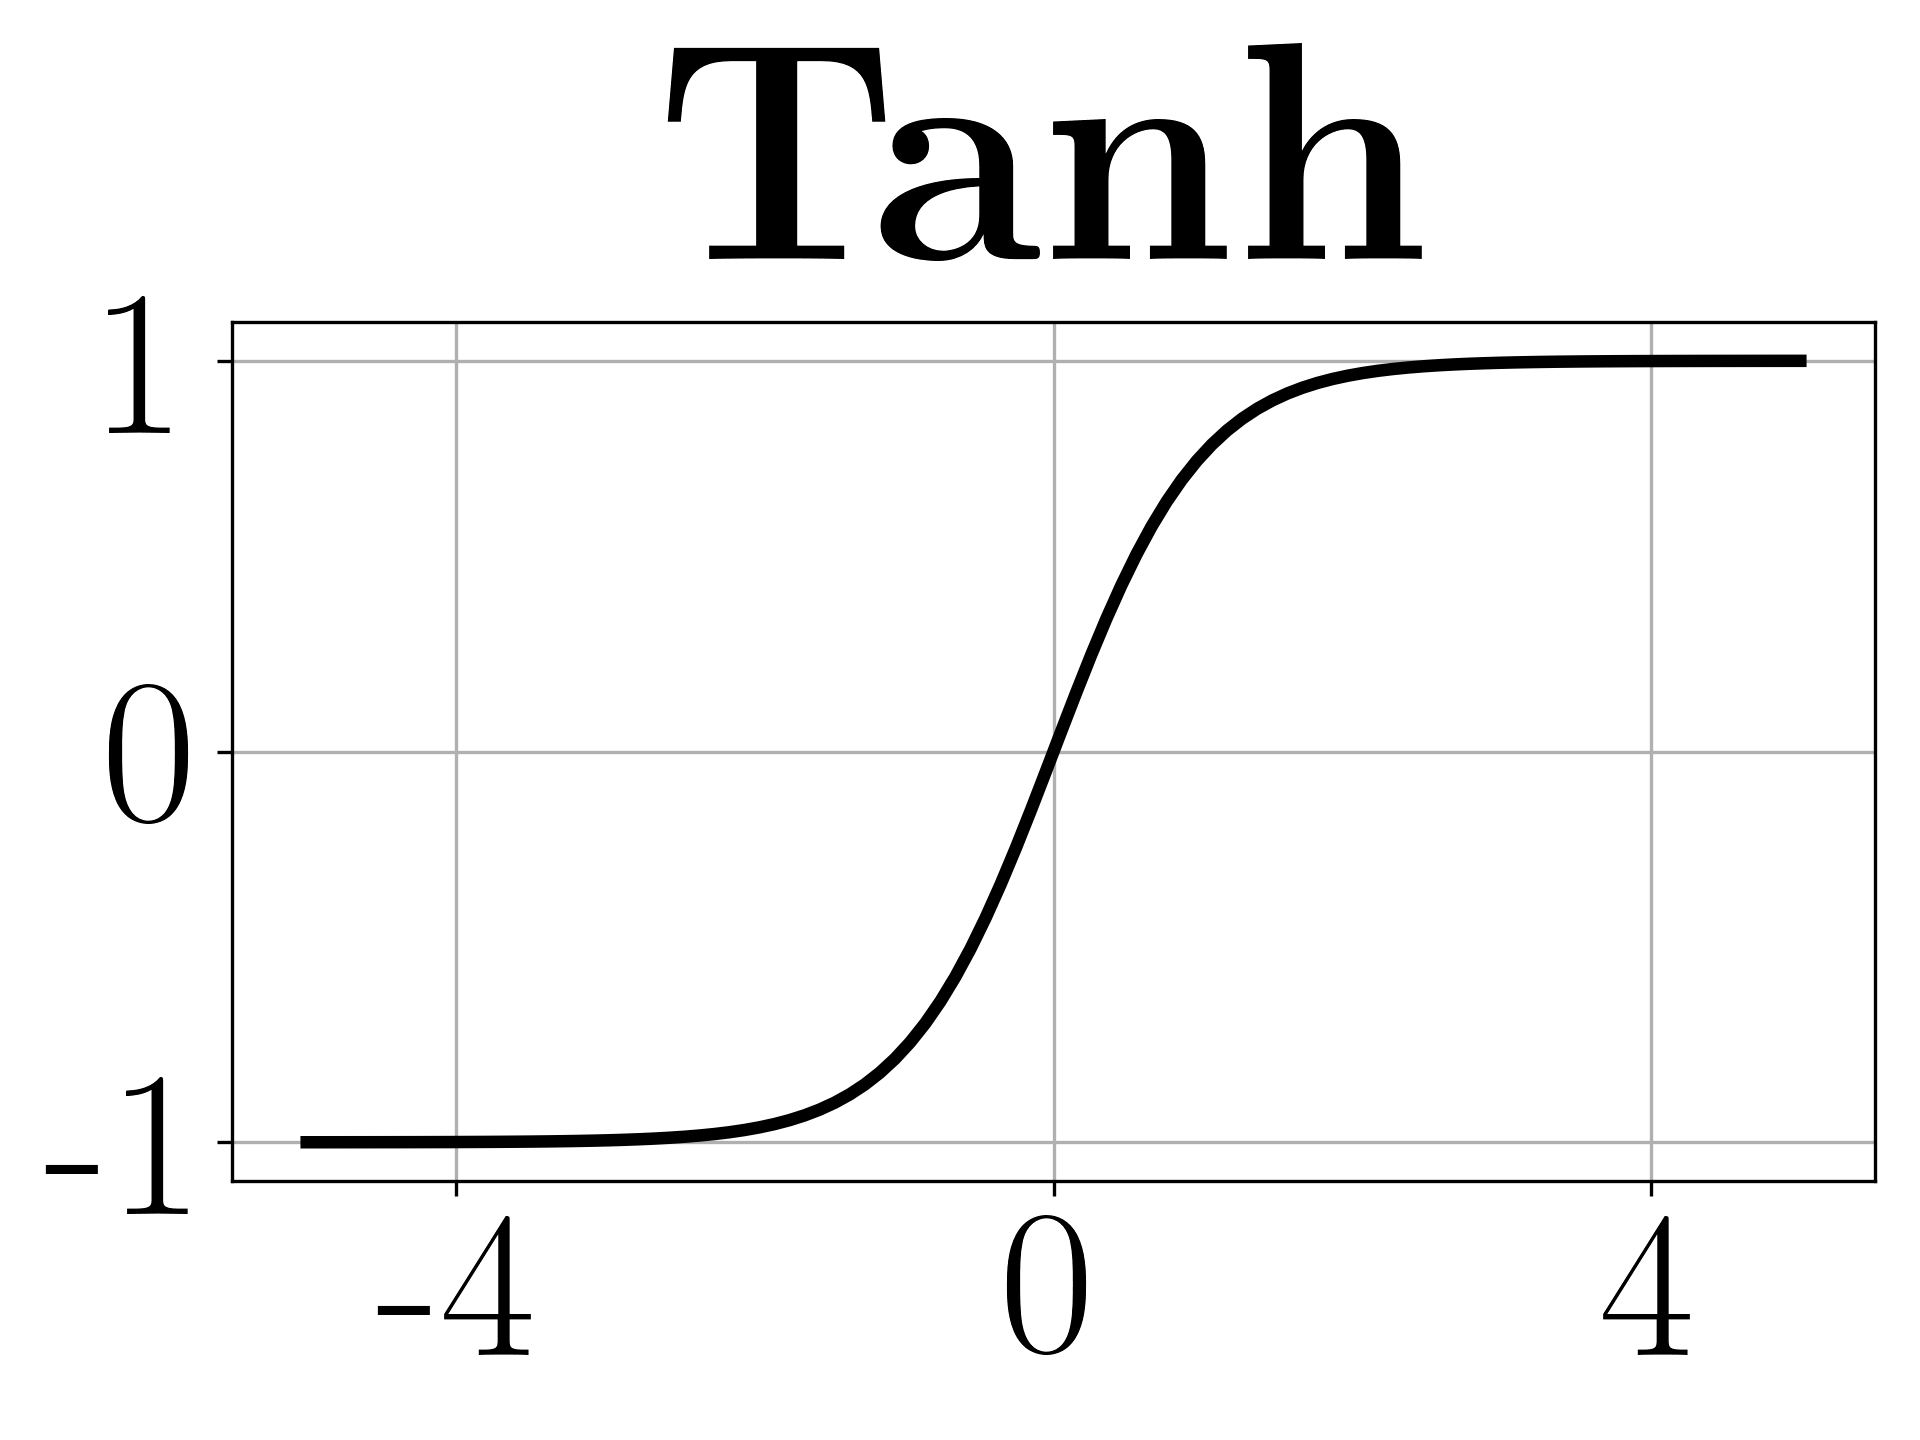
\includegraphics[width=.1\textwidth]{margarine/figs/tanh_function.png}};
        
        \node[bluenode, below left=of hl2, text width=0.5cm, align=center, yshift=0.3cm](input_2) {$\theta_2$};
        \node[bluenode, above=of input_2, text width=0.5cm, align=center, yshift=0.12cm](input_1) {$\theta_1$};
        \node[bluenode, below=of input_2, text width=0.5cm, align=center, yshift=0.1cm](input_3) {$\theta_3$};

        \node[greennode, right=of 0, text width=0.5cm, align=center, yshift=0.3cm](output_2) {$z^\prime_2$};
        \node[greennode, above=of output_2, text width=0.5cm, align=center, yshift=0.12cm](output_1) {$z^\prime_1$};
        \node[greennode, below=of output_2, text width=0.5cm, align=center, yshift=0.1cm](output_3) {$z^\prime_3$};
        
        \node[right=of output_2, align=left, xshift=-1.5cm, yshift=0.12cm] {$= (\theta_2 -\mu_2) / \sigma_2$};
        
        \node[right=of output_1, align=left, xshift=-1.5cm, yshift=0.12cm] {$= (\theta_1 -\mu_1) / \sigma_1$};
        
        \node[right=of output_3, align=left, xshift=-1.5cm, yshift=0.12cm] {$= (\theta_3 -\mu_3) / \sigma_3$};
        
        \draw[densely dashed](input_1.east) -- (output_1.west);
        
        \draw[densely dashed](input_2.east) -- (output_2.west);
        
        \draw[densely dashed](input_3.east) -- (output_3.west);
        
        \draw[->](input_1.east) -- (hl1.west);
        \draw[->](input_1.east) -- (hl2.west);
        \draw[->](input_1.east) -- (hl3.west);
        \draw[->](input_1.east) -- (hl4.west);
        
        %\draw[->](input_2.east) -- (hl1.west);
        %\draw[->](input_2.east) -- (hl2.west);
        \draw[->](input_2.east) -- (hl3.west);
        \draw[->](input_2.east) -- (hl4.west);
        
        %\draw[->](input_3.east) -- (hl1.west);
        %\draw[->](input_3.east) -- (hl2.west);
        %\draw[->](input_3.east) -- (hl3.west);
        %\draw[->](input_3.east) -- (hl4.west);
        
        \draw[->](hl1.east) -- (layer1_center1.west);
        \draw[->](hl2.east) -- (layer1_center1.west);
        %\draw[->](hl3.east) -- (layer1_center1.west);
        %\draw[->](hl4.east) -- (layer1_center1.west);
        
        \draw[->](hl1.east) -- (layer1_center2.west);
        \draw[->](hl2.east) -- (layer1_center2.west);
        %\draw[->](hl3.east) -- (layer1_center2.west);
        %\draw[->](hl4.east) -- (layer1_center2.west);
        
        %\draw[->](hl1.east) -- (layer1_top1.west);
        %\draw[->](hl2.east) -- (layer1_top1.west);
        %\draw[->](hl3.east) -- (layer1_top1.west);
        %\draw[->](hl4.east) -- (layer1_top1.west);
        
        %\draw[->](hl1.east) -- (layer1_top2.west);
        %\draw[->](hl2.east) -- (layer1_top2.west);
        %\draw[->](hl3.east) -- (layer1_top2.west);
        %\draw[->](hl4.east) -- (layer1_top2.west);
        
        \draw[->](hl1.east) -- (layer1_bottom2.west);
        \draw[->](hl2.east) -- (layer1_bottom2.west);
        \draw[->](hl3.east) -- (layer1_bottom2.west);
        \draw[->](hl4.east) -- (layer1_bottom2.west);
        
        \draw[->](hl1.east) -- (layer1_bottom1.west);
        \draw[->](hl2.east) -- (layer1_bottom1.west);
        \draw[->](hl3.east) -- (layer1_bottom1.west);
        \draw[->](hl4.east) -- (layer1_bottom1.west);
        
        \draw[densely dashed](layer1_top1.east) -- (output_1.west);
        \draw[densely dashed](layer1_top2.east) -- (output_1.west);
        
        \draw[densely dashed](layer1_center1.east) -- (output_2.west);
        \draw[densely dashed](layer1_center2.east) -- (output_2.west);
        
        \draw[densely dashed](layer1_bottom1.east) -- (output_3.west);
        \draw[densely dashed](layer1_bottom2.east) -- (output_3.west);

    \end{tikzpicture}
    \caption{The Masked Autoencoder for Distribution Estimation~(MADE) architecture, when trained appropriately, transforms samples from a complex probability distribution $\{\theta\}$ on to samples from a standard normal distribution under the assumption that the probability distribution $\{\theta\}$ can be broken into conditional one-dimensional Gaussian probability distributions. Many different MADE networks can be stacked together and trained to produce a normalising flow increasing the expressivity of the density estimation. By definition, normalising flows are bijective, and a trained implementation can be used to calculate $\log(P(x))$ and draw samples from $P(x)$. }
    \label{fig:maf}
\end{figure*}

By chaining a series of these networks together, we create a MAF. This improves the expressivity of the emulator and can be expressed using the following formalism
\begin{equation}
    \begin{split}
    z_0 & = \mathcal{N}(0, 1) \\
    z_1 & = z_0 \sigma_1(z_0, w_1) + \mu_1(z_0, w_1)\\
    \vdots &\\
    x & = z_{n-1} \sigma_{n}(z_{n-1}, w_{n-1}) + \mu_{n}(z_{n-1}, w_{n-1})
    \end{split}
\label{eq:MAF}
\end{equation}
where the index here refers to a given network in the chain. We train the chain of neural networks simultaneously with one loss function and feed the outputs of proceeding networks into subsequent networks in the chain. 

\end{comment}

To improve the accuracy of the density estimation, we can transform the target posterior samples that we input to our MAF into a Gaussian parameter space via the standard normal cumulative distribution function~(CDF). The target distribution in this normalised space is a skewed and scaled version of the base distribution $z_0$ which makes the transformation easier to learn.

Due to the invariance of the KL divergence and, similarly, the BMD under a change of variables, we can calculate their values in any transformed version of the original parameter space provided the prior and posterior undergo the same change of variables. In practice, \textsc{margarine} calculates these quantities in the gaussianized space. A uniform prior in the gaussianized space corresponds to the standard normal distribution. For more complex priors, we can transform them into this space in the same way we transform the posteriors and train a prior MAF to calculate the marginal Bayesian statistics.

There are a number of tunable parameters involved when designing MAFs including the number of networks, the number of layers in each network, the number of epochs and the learning rate. All of these parameters can be explored using \textsc{margarine}, and we use recommendations from a previous implementation~\cite{Alsing_bijectors_2021}.

\subsection{Kernel Density Estimation}

A simple 1D Kernel Density Estimator~(KDE) is defined by
\begin{equation}
    \mathcal{P}(x) = \frac{1}{nh}\sum_{i=1}^n K\bigg(\frac{x-x_i}{h}\bigg)
    \label{eq:gauss_kde}
\end{equation}
where $h$ is known as the bandwidth, $K$ is the kernel and $n$ the number of samples in the set $x$. This scales to higher dimensions where $x$ and $x_i$ become $N$ dimensional vectors and $h$ becomes a 2D matrix of bandwidths. We use a multivariate Gaussian kernel where $h$ is equivalent to the covariance matrix and $x_i$ is equivalent to an $N$ dimensional vector of means. Since the KDE is a sum of known kernels with a known covariance matrix and set of means, then the probability distribution of the samples is trivially calculable, as is its logarithm.

When generating KDEs, we perform the same type of normalisation of our target distribution as is done with the MAFs, transforming it into a Gaussianised space via a standard normal CDF. The transformation allows the density estimator to better capture the edges of very flat and uniform posteriors.

We can generate samples from trained KDEs and calculate marginal Bayesian statistics, however KDEs are not strictly bijective. Adapting a KDE to be bijective is a non-linear process and requires the use of a root-finding algorithm to transform from the hypercube to the KDE space. This is a process that is not currently optimized, but is fully implemented in \textsc{margarine} allowing the user to generate KDE priors.

To transform the unit hypercube into samples on the target distribution via the KDE we first note that KDEs model the target probability distribution by breaking it down into the product of conditional probabilities
\begin{equation}
    P(x_1, x_2, \hdots, x_n) = P(x_1) P(x_2|x_1) \hdots P(x_n | x_1, x_2, \hdots, x_{n-1})
\end{equation}
modelled by a Gaussian kernel at each data point. We then use the inverse CDFs of each Gaussian conditional probability to transform samples on the hypercube to samples on the target distribution
\begin{equation}
    (u_1, u_2, \hdots, u_n) \rightarrow (x_1, x_2, \hdots, x_n),
\end{equation}
via
\begin{equation}
    \begin{split}
       x_1 & = F_1(u_1) \\
        x_2 & = F_2(u_2;x_1) \\
        \vdots & \\
       x_n & = F_n(u_n;x_1, x_2, \hdots, x_{n-1})
    \end{split}
\end{equation}
where $F_i$ are the conditional and marginalised inverse CDFs. 

For a multivariate Gaussian KDE, marginalisation is equivalent to ignoring components of $h$ and $x_i$ in the multivariate equivalent of \cref{eq:gauss_kde}. Conditioning the probability distribution simply involves analytical corrections to the means and standard deviations based on the corresponding values for the $n-1$ distributions. The equivalent transformation using MAFs is much more computationally efficient. There are fewer tunable parameters for the KDE, however we can change the bandwidth of the kernel. We use the Silverman~\cite{silverman2018density} approach to calculate $h$ but note that this can be modified with \textsc{margarine}.

\section{Applications of \textsc{margarine}}
\label{sec:applications}

\subsection{Nuisance-Free Likelihood}
\label{sec:nuisance_free_likelihood_apps}

\subsubsection{Toy 21-cm Example}

To illustrate the application of the nuisance free likelihood function, we use an example from 21-cm cosmology.
To a crude approximation, the 21-cm signal can be modelled with a Gaussian absorption profile. %For a review of the physics of the 21-cm signal see \cite{Furlanetto_review_2006, Mesinger2019}
We generate two different mock sky-averaged 21-cm data sets with different bandwidths of $50- 100$ and $75 - 190$~MHz with different foregrounds to simulate observations from different locations. We call these two experiments $A$ and $B$ and model the foreground as
\begin{equation}
    T_\mathrm{fg} = a \nu^{-\beta},
\end{equation}
where $a$ is a common scaling factor for both experiments and $\beta$ is set as $-2.6$ and $-2.5$. The model is based on the expectation that the foreground is composed of smooth synchrotron and free-free emission and the power law is based on observational constraints from experiments like EDGES~\citep{Mozdzen_EDGES_spectral_index_2017}, SARAS3~\citep{SARAS3}, and LEDA \citep{LEDA_spectral_Index_2021}.

%It's typical in 21-cm experiments to model the foreground as an unconstrained polynomial function due to its smooth properties. However, the structure of the antenna beam can introduce non-smooth chromatic features into the data and more complex forward modelling of the foreground is need. 
For simplicity, we assume an achromatic beam for each experiment and thus a data set that includes a smooth foreground and Gaussian 21-cm signal. The signal in our mock data is given by
\begin{equation}
    T_{21} = - T_\mathrm{min} \exp\bigg(-\frac{(\nu - \nu_c)^2}{2\Delta \nu ^2}\bigg),
    \label{eq:gaussian_signal}
\end{equation}
where $T_\mathrm{min}$ is the signal amplitude, $\nu$ is the frequency range of the data, $\nu_c$ is the central frequency of the absorption feature and $\Delta \nu$ is the signal's width. We set $T_\mathrm{min} = 0.25$~K, $\nu_c = 80$~MHz and $\Delta \nu = 10$~MHz.

We explore each likelihood separately with the Nested Sampling algorithm \textsc{polychord}, \cref{eq:gaussian_signal} and a log-log polynomial foreground model given by
\begin{equation}
    \log_{10}(T_\mathrm{fg}) = \sum^{N}_{i=0} a_i \log_{10}(\nu)^{i},
\end{equation}
where $a_i$ are coefficients to be fitted. In practice, the foreground modelling is not always consistent across different data sets and to further emphasise that the two mock experiments are observing different parts of the sky, we assume they have different complexities and fit a 3-term polynomial to experiment $A$ and a 4-term polynomial to experiment $B$ for the foreground. Generally, when polynomials are being used, the order of the polynomial would be optimised through the assessment of the Bayesian evidence. We inject Gaussian random noise into our data sets with standard deviations of $35$~mK and $15$~mK for experiments $A$ and $B$ respectively.

In our Nested Sampling runs, we use a Gaussian log-likelihood function
\begin{equation}
    \log\mathcal{L} = \sum_i \bigg(-\frac{1}{2}\log(2\pi \sigma^2) -\frac{1}{2}\bigg(\frac{T_\mathrm{D}(\nu_i) - T_\mathrm{fg}(\nu_i) - T_{21}(\nu_i)}{\sigma}\bigg)^2\bigg),
\end{equation}
where $T_D$ corresponds to the mock data and $\sigma$ corresponds to the instrument noise and is a modelled parameter. In the top panels of \cref{fig:joint_likelihood} we show the sum of the noise and signal models that went into the mock datasets and the functional averages of our fitted 21-cm signals
\begin{equation}
    \overline{T_{21}} = \frac{\sum_i^{N_\mathrm{samples}} w_i T_{21}(\theta_{21, i})}{\sum_i^{N_\mathrm{samples}} w_i}
\end{equation}
where $w_i$ is the weight corresponding to sample $i$ output by \textsc{polychord}.

We also show in the center right panel of \cref{fig:joint_likelihood} the resultant $\overline{T_{21}}$ found fitting both data sets simultaneously with
\begin{equation}
    \log \mathcal{L}_\mathrm{A,B} (\theta, \alpha_{A}, \alpha_B) =  \log \mathcal{L}_\mathrm{A} (\theta, \alpha_A)~+ \\ \log \mathcal{L}_\mathrm{B} (\theta, \alpha_B).
\end{equation}
Through the combination of the two data sets we can see by visual inspection that we get a much better fit to the data than is achieved for each experiment individually as is to be expected.

However, in order to do this we have had to sample over the nuisance parameters, $\alpha_A$ and $\alpha_B$ (e.g. \cref{fig:pipeline}). Alternatively, with \textsc{margarine} we can generate nuisance-free likelihood functions for each experiment and sample
\begin{equation}
    \log \mathcal{L}_\mathrm{A,B} (\theta) = \log \mathcal{L}_\mathrm{A} (\theta)~+ \log \mathcal{L}_\mathrm{B} (\theta),
\end{equation}
over just the parameters of our 21-cm model without having to consider modelling the foregrounds (e.g. \cref{fig:pipelineB}).

We show the resultant $\overline{T_{21}}$ from the joint analysis with \textsc{margarine} in the center left panel of \cref{fig:joint_likelihood} and we can see that the fit is consistent with the more complex analysis. In particular, we note the approximate consistency between the Bayesian evidences for each fit. The error on the evidence for the \textsc{margarine} fit is likely underestimated due to uncertainty in the density estimation, however this is currently hard to quantify and left for future work.

\begin{figure}
    \centering
    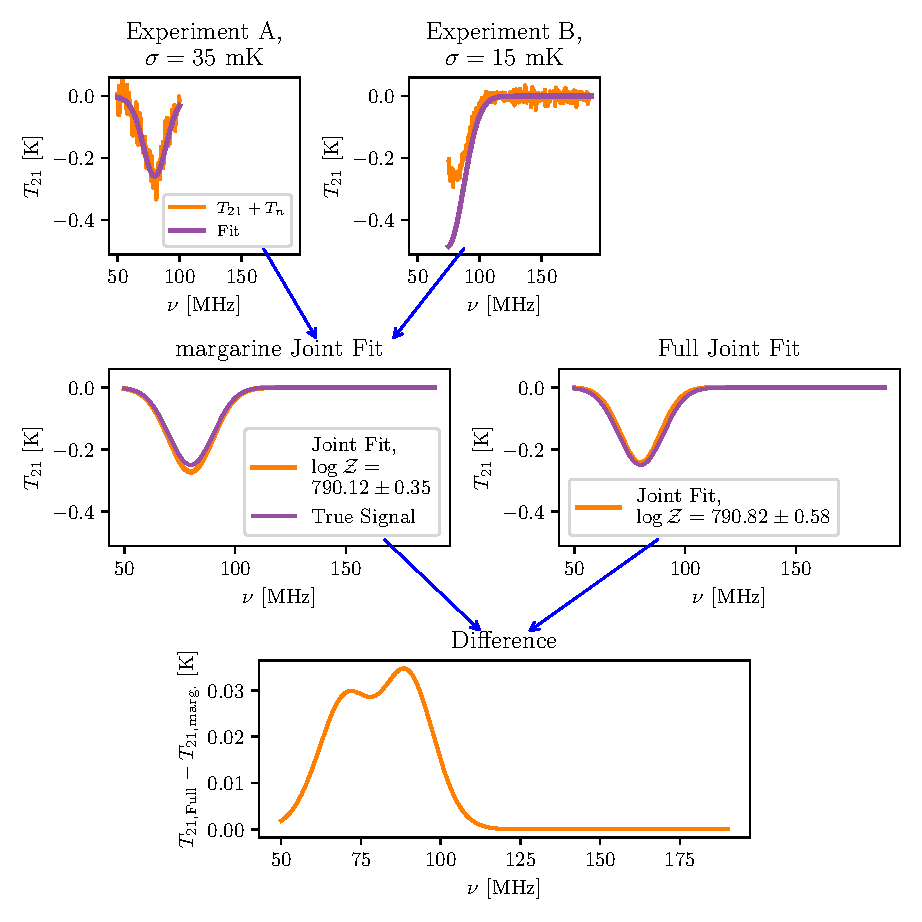
\includegraphics{margarine/figs/margarine_combined_signal.pdf}
    \caption{The top panels in the graph shows two simulated data sets comprising noise and a 21-cm signal as orange lines. In the same panels in purple, we show the averages of the functional posteriors derived from Nested Sampling fits to both of these data sets. Neither fit recovers the true signal exactly, however when we analytically combine the full likelihoods for each experiment, including foregrounds, and jointly fit the data we get a much better agreement across the whole frequency range as can be seen in the center right panel. We show the results of this joint analysis as a purple line. For comparison, we show in the center left panel, as an orange line, the average of the functional posterior from a joint fit performed with \textsc{margarine} using the nuisance-free likelihood function. We can see that the joint fits are equivalent, more accurate than the fits to each individual experiment and the Bayesian evidences are similar in magnitude when using the full likelihood and the nuisance-free likelihood. We show the difference between the two fits in the bottom panel as a function of frequency.}
    \label{fig:joint_likelihood}
\end{figure}

In this case because the problem is trivial sampling over $\theta$, $\alpha_A$ and $\alpha_B$ is not an inefficient or complex process, however generally speaking there are many more nuisance parameters that need to be modelled and the complexity of those models can significantly increase the evaluation time per call to the likelihood \citep[e.g. \cref{ch:saras2}, ][]{Bevins_SARAS2_2022}. In these circumstances, \textsc{margarine} can act as a useful tool for efficiently combining constraints from different data sets \citep[e.g. \cref{ch:hera_saras3}, ][]{Bevins_hera_saras3_2023} and this is discussed further in the next section.

\subsubsection{Combining constraints from Planck and DES}
\label{sec:results}

%It has previously been demonstrated that \textsc{margarine} is capable of replicating complex probability distributions and approximating marginal Bayesian statistics such as the KL divergence and the BMD \cite{margarine_neurips}. Here we demonstrate the theory discussed in \cref{sec:theory} by 
Here we combine samples from the Dark Energy Survey~(DES) Year 1 posterior \cite{DES_Year1_2018} and Planck posterior \cite{Planck2018} using \textsc{margarine} to estimate nuisance-free likelihoods. DES surveys supernovae, galaxies and large scale cosmic structures in the universe in an effort to measure dark matter and dark energy densities and model the dark energy equation of state. In contrast, Planck mapped the anisotropies in the Cosmic Microwave Background~(CMB) and correspondingly provided constraints on key cosmological parameters.

The constraints from DES and Planck have previously been combined using a full Nested Sampling run over all parameters including a multitude of `nuisance' parameters in a computationally expensive exercise \cite{Handley_tensions_2019} (e.g. \cref{fig:pipeline}). %This corresponds to the flow chart in \cref{fig:pipeline} and 
The previous analysis gives us access to the combined DES and Planck evidence, which is found to have a value of $\log(\mathcal{Z}) = -5965.7 \pm 0.3$. In \cref{fig:joint} we show the DES, Planck and joint posteriors for the six cosmological parameters derived in this work using \textsc{margarine} and the flow chart in \cref{fig:pipelineB}. The constrained parameters are the baryon and dark matter density parameters, $\Omega_b h^2$ and $\Omega_c h^2$, the angular size of the sound horizon at recombination, $\theta_{MC}$, the CMB optical depth, $\tau$, the amplitude of the power spectrum, $A_s$, and the corresponding spectral index, $n_s$. These make up the set $\theta = (\Omega_b h^2, \Omega_c h^2, \theta_{MC}, \tau, A_s, n_s)$. We use the Nested Sampling algorithm \textsc{polychord} in our analysis \cite{Handley2015a, Handley2015b}.

We use a uniform prior that is defined to be three sigmas around the Planck posterior mean. This is done to improve the efficiency of our Nested Sampling run. However, we subsequently have to re-weight the samples and correct the evidence for the difference between the priors used here and in the previous full Nested Sampling run \cite{Handley_tensions_2019} for comparison. If we define
\begin{equation}
    \mathcal{Z}_A = \int \mathcal{L}(\theta) \pi_A(\theta) d\theta, \qquad
    \mathcal{Z}_B = \int \mathcal{L}(\theta) \pi_B(\theta) d\theta, 
\end{equation}
where $A$ is our uniform prior space and $B$ is our target prior space from the previous work \cite{Handley_tensions_2019}, then
\begin{equation}
    \mathcal{Z}_B 
    = \int \mathcal{L}(\theta) \pi_B(\theta) d\theta
    = \int \mathcal{L}(\theta) {\pi_A(\theta)}\frac{\pi_B(\theta)}{\pi_A(\theta)} d\theta 
   = \mathcal{Z}_A\left\langle \frac{\pi_B(\theta)}{\pi_A(\theta)}\right\rangle_{\mathcal{P}_A}
\end{equation}
giving
\begin{equation}
    \mathcal{Z}_B 
    = \mathcal{Z}_A\left\langle \frac{\pi_B(\theta)}{\pi_A(\theta)}\right\rangle_{\mathcal{P}_A}.
\end{equation}
Then following similar arguments we can transform our posteriors by re-weighting the distributions with the following
\begin{equation}
    w^{(i)}_B 
    = w^{(i)}_A  \frac{\pi_B(\theta^{(i)})}{\pi_A(\theta^{(i)})}.
\end{equation}

We see from the figure and corresponding table that with our joint analysis we are able to derive a log-evidence that is approximately consistent with that found in \cite{Handley_tensions_2019}, $\log(\mathcal{Z}) = -5965.7 \pm 0.3$ as previously reported, further validating the theory discussed and its implementation with \textsc{margarine}. %We note that the re-weighting described above relies on calculation of the two prior log-probabilities for which we use \textsc{margarine} and currently do not have an estimate of the error for. As a result, the error in the combined evidence, $Z_B$, is given by the error in $Z_A$ from the nested samples and is likely underestimated. 
Using \textsc{margarine} we can also derive the combined KL divergence, also reported in \cref{fig:joint} and discussed further in this chapter, which we find is consistent with the result in the literature of $\mathcal{D} = 6.17 \pm 0.36$ \cite{Handley_dimensionality_2019}. Similarly, we derive marginal KL divergences for the DES and Planck cosmological parameters using \textsc{margarine} (the DES example is furthered in the following subsections). A full discussion of the implications of combining the two data sets for our understanding of cosmology can be found in the literature \cite[e.g][]{Handley_tensions_2019, Handley_dimensionality_2019}.

By reducing the number of parameters that need to be sampled, we significantly reduce the Nested Sampling runtime. For \textsc{polychord} the runtime scales as the cube of the number of dimensions \cite{supernest}. This can be seen by assessing the time complexity of the algorithm where, $T \propto n_\mathrm{live} \times \langle T\{\mathcal{L}(\theta)\}\rangle \times \langle T\{Impl.\}\rangle \times \mathcal{D}(\mathcal{P}||\pi)$. Here $n_\mathrm{live}$ scales with the number of dimensions, $d$, as does the Kullback-Leibler divergence. For \textsc{polychord}, the specific implementation time complexity factor, $\langle T\{Impl.\}\rangle$, representing the impact of replacing dead points with higher likelihood live points on the runtime, scales linearly with $d$. Together this gives $T \propto d^3 \times \langle T\{\mathcal{L}(\theta)\}\rangle$. Therefore, by using nuisance-free likelihoods and sampling over 6 parameters rather than 41 parameters (cosmological plus 20 nuisance parameters for DES and 15 different nuisance parameters for Planck) we reduce the runtime by a factor of $(41/6)^3 \approx 319$ with further improvements in $\langle T\{\mathcal{L}(\theta)\}\rangle$. %Using \textsc{margarine}, $\langle T\{\mathcal{L}(\theta)\}\rangle$ is typically reduced since analytic likelihoods are computationally more expensive than emulated likelihoods.

\begin{figure}
    \centering
    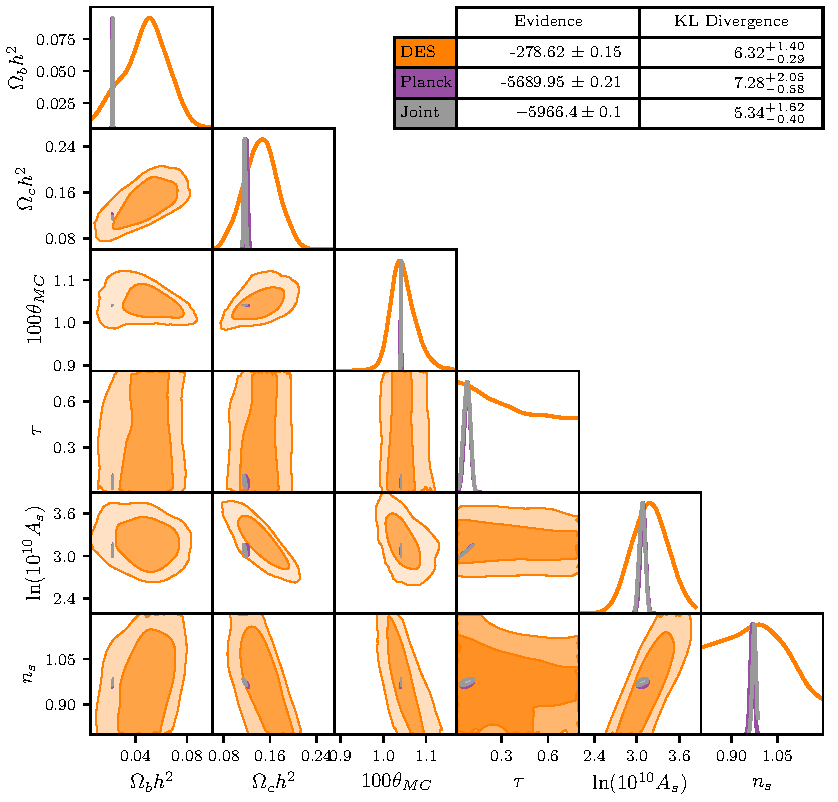
\includegraphics{margarine/figs/paper_plot.pdf}
    \caption{The combined posterior (in grey) found when combining the constraints on the cosmological parameters from DES and Planck using \textsc{margarine}. For DES and Planck, we calculate the marginal KL divergences using \textsc{margarine}, whereas the Bayesian evidences are calculated using \textsc{anesthetic}. The joint evidence and joint KL divergence are calculated with a combination of the two codes and are found to be approximately consistent with those found in the literature \cite{Handley_tensions_2019, Handley_dimensionality_2019}. Note that the error on the joint evidence is likely underestimated as it relies on evaluations of log-probabilities for various distributions, for which \textsc{margarine} does not currently provide errors. The figure produced with \textsc{anesthetic} \cite{anesthetic}.}
    \label{fig:joint}
\end{figure}

\subsection{Prior Emulation}

Since the 21-cm signal is dependent on many different astrophysical process, semi-numerical simulations can take several hours to produce a single model. This is impractical if we want to use Bayesian inference techniques like MCMC and Nested Sampling algorithms to fit real data. Signal emulators, like those discussed in the previous chapter, are often used as a fast alternative that can accurately model the relationship between the astrophysics and the signal structure and produce signal realisations in 10s of milliseconds. An even cheaper alternative is to approximate the signal with a Gaussian absorption feature, as alluded to in the previous section. However, it is not always clear how to set the priors on the parameters $T_\mathrm{min}$, $\nu_c$ and $\Delta \nu$ in \cref{eq:gaussian_signal}. For this, we can use \textsc{margarine}.

The idea here is to take a large set of physically motivated signals generated using an emulator from a uniformly sampled prior on the astrophysical parameters describing the underlying semi-numerical simulation. For each physical signal we then calculate the depth corresponding to $T_\mathrm{min}$, the central frequency $\nu_c$ and approximate the width $\Delta \nu$. Through this process we arrive at a physically motivated set of samples in the phenomenological parameters which we can train a MAF on using \textsc{margarine}, creating a physically motivated prior on our phenomenological parameters.

We use the global 21-cm signal emulator \textsc{globalemu} \citep{Bevins_globalemu_2021}, discussed in \cref{ch:globalemu}, to model a set of 5,000 signals based on a parameterisation of the signal that includes; $V_c$ the minimum virial circular velocity that is proportional to the cube root of the halo mass for star formation, $f_*$ the star formation efficiency, $f_X$ is the X-ray production efficiency which is proportional to the X-ray luminosity, $\tau$ the CMB optical depth and $f_r$ the radio production efficiency proportional to the radio luminosity \cite{Reis2020}.
Whilst 5,000 signals may seem like a large number of models, the equivalent number generated in a Nested Sampling or MCMC run would be far larger.

In scenarios with poor star formation, corresponding to high $V_c$ and low $f_*$, and large X-ray heating corresponding to high $f_X$ we find that the signal cannot be well approximated by a Gaussian profile because it features a weak absorption feature and strong emission. We therefore filter out these scenarios before training our MAF and of the 5,000 models we initially started with, 87\% are used to produce our physically motivated prior. In \cref{fig:physical_prior} we show the distribution on $\log_{10}(|T_\mathrm{min}|)$, $\nu_c$ and $\Delta \nu$ generated from the physical models and samples from the corresponding MAF which can be used as a prior on the Gaussian model.

In 21-cm cosmology, instrumental effects can introduce non-smooth structure to the data. These effects are often sinusoidal \citep[e.g.][]{Bevins_maxsmooth_2021, Bevins_SARAS2_2022} and if not corrected for they can affect the recovery of the 21-cm signal. For example, part of a damped sinusoidal structure in the data with a periodicity of 5~MHz can be modelled with the approximate Gaussian signal profile discussed in this chapter if the prior on the width is wide. However, from \cref{fig:physical_prior} we see that a signal profile of width 5~MHz is not likely to represent a physical scenario. The goal of the physically motivated prior is to therefore provide some information about the anticipated signal that can help to separate it from and prevent fitting systematic structures in the data when using a Gaussian profile for the signal.

\begin{figure*}
    \centering
    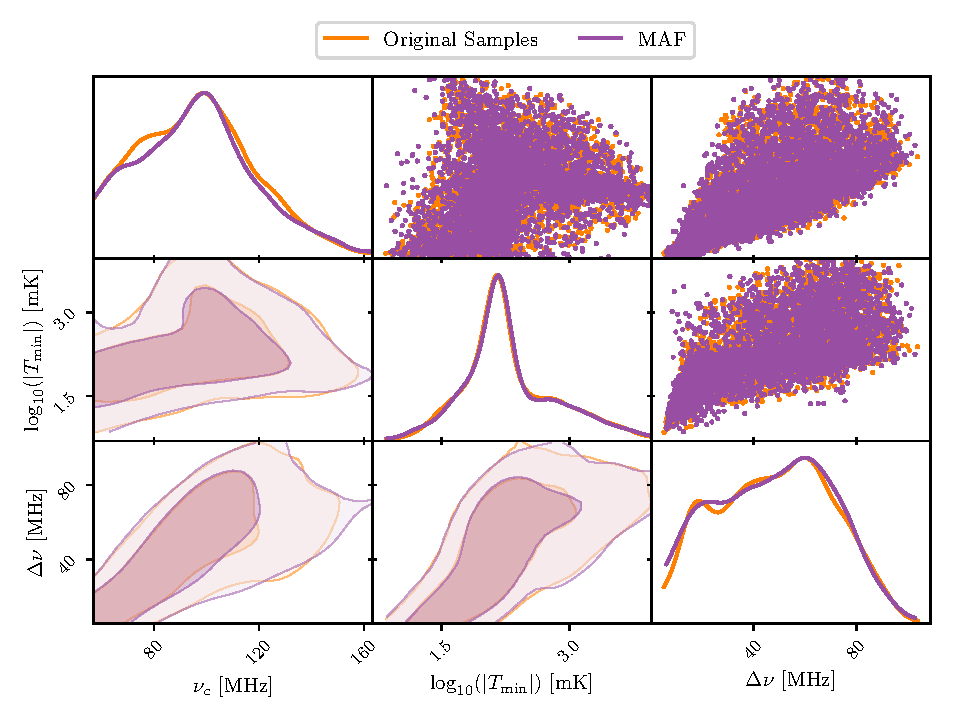
\includegraphics{margarine/figs/physical_prior_example.pdf}
    \caption{A physically motivated prior on the phenomenological parameters of a Gaussian absorption feature used to model the sky-averaged 21-cm signal. $\nu_c$ is the central frequency of the absorption feature, $T_\mathrm{min}$ is the corresponding temperature, and $\Delta \nu$ is the approximate width of the 21-cm signal. The prior is derived by approximating the phenomenological parameters for a set of physically motivated signals generated with a neural network emulator and learning the corresponding distribution, in orange, with a MAF. Samples from the MAF are shown in purple.}
    \label{fig:physical_prior}
\end{figure*}

\subsection{Marginal Bayesian Statistics}
\subsubsection{Toy Example Posteriors}

We use two different toy examples for which we know the KL divergence and BMD to demonstrate the calculation of marginal Bayesian statistics. We sample the example Gaussian likelihoods, both with five parameters, using \textsc{polychord}, and we show the corresponding distributions in orange in \cref{fig:toy_example}. The first has a series of correlations between the parameters (left-hand panel) and the second has a combination of uncorrelated parameters with both log-uniform and uniform priors on the parameters (right-hand panel).

\begin{figure*}
    \centering
    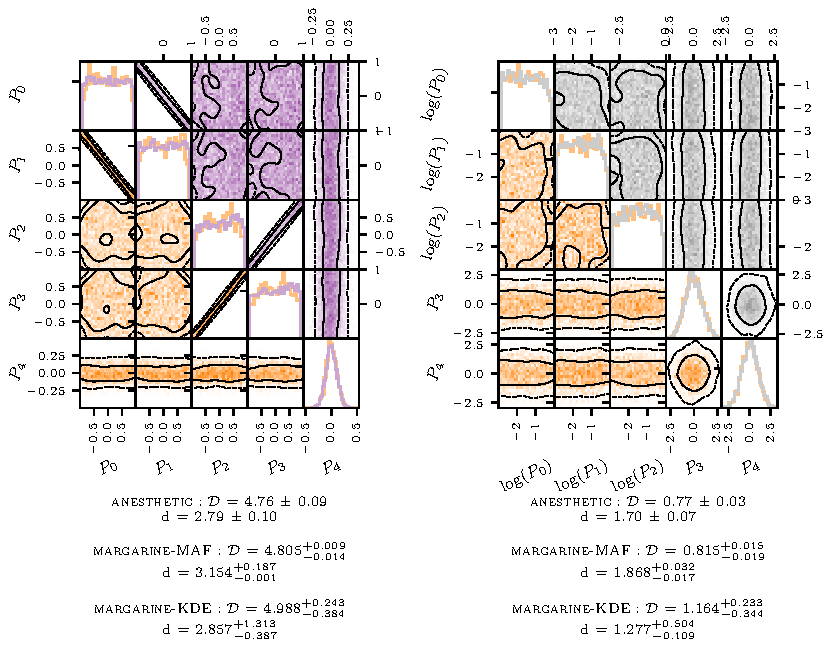
\includegraphics[width=\linewidth]{margarine/figs/toy_examples_alt.pdf}
    \caption{\textbf{Left Panel:} The graph shows a set of correlated nested samples from \textsc{polychord} in orange along with a reconstruction from a trained KDE in purple. Listed are the corresponding `true' values for the KL divergence and BMD from \textsc{anesthetic} and the estimated values from \textsc{margarine} using both a KDE and MAF. \textbf{Right Panel:} An equivalent graph for a set of uncorrelated samples with both log-uniform and uniform priors on the parameters, shown in orange. The gray samples are taken from a trained MAF, and we report the `true' Bayesian statistics values from \textsc{anesthetic} along with estimates calculated using a MAF and KDE with \textsc{margarine}.}
    \label{fig:toy_example}
\end{figure*}

We are able to use the samples from \textsc{polychord} and the analysis tool \textsc{anesthetic}~\cite{anesthetic} to calculate the KL divergence and BMD for both toy examples and these values are reported, with errors, in \cref{fig:toy_example}. We show samples drawn from a KDE trained on the correlated samples and from a MAF trained on the uncorrelated samples, with values of $\mathcal{D}$ and $d$ listed for both types of density estimator.

The errors in $\mathcal{D}$ and $d$ are estimated by propagating both samples generated with the density estimator and the original samples through the density estimator to evaluate the log-probabilities and comparing the resultant statistics. If the density estimator is a perfect representation of the original distribution, then we would expect samples drawn from it to be from the same distribution as the original samples. This would lead to an approximate equivalence between the two sorted log-probability distributions as functions of the sorted associated Nested Sampling weights~\cite{Harrison2015} and so any deviation we see gives us an indication of the error in our marginal statistics.

For the correlated samples, we see that the estimated KL divergence and BMD from the MAF and from the KDE are in close agreement with the `true' value output from \textsc{anesthetic}.
For the uncorrelated samples, we also see that the MAF KL divergence and BMD estimates are in agreement with the \textsc{anesthetic} values. For the KDE, the KL divergence and BMD are less consistent with the values from the MAF and from \textsc{anesthetic}, however we find we have larger errors when using the KDEs likely because they are less expressive than the MAFs. 

Typically, the upper and lower bounded range on the BMD estimates are larger than for the KL divergence estimates because it has a more complex dependence on $\log\mathcal{L}$. Future work is needed to investigate whether improvements can be made to the BMD estimates by modifying the MAF loss function, network configurations or KDE bandwidths among other tunable parameters.

\subsubsection{Radio Experiment for the Analysis of Cosmic Hydrogen}

%The Radio Experiment for the Analysis of Cosmic Hydrogen~(REACH) is an experiment aiming to detect the sky-averaged 21-cm signal in the frequency range $50 - 170$ MHz.

The Radio Experiment for the Analysis of Cosmic Hydrogen~(REACH)  data analysis pipeline \cite{Anstey_REACH_2021} uses Nested Sampling, implemented with \textsc{polychord}, to model the different components of the data. The pipeline has been extensively tested on mock observations~\citep{Anstey_REACH_2021,Anstey_antenna_2022,Cumner_antenna_2021, Scheutwinkel2022a, Scheutwinkel2022b}. We generate mock observational data using a realistic foreground model derived from an all-sky map and inject a Gaussian signal profile with an amplitude of $|T_\mathrm{min}| = 155$~mK, a central frequency of $\nu_c = 85$~MHz and a standard deviation of $\Delta \nu = 15$~MHz.

The mock data correspond to a single snapshot observation taken from the Karoo radio observatory with a dipole antenna and modelled with a foreground model that takes advantage of the spectral structure of the sky, a correction for the non-uniform response of the antenna to the sky, Gaussian noise and a Gaussian signal profile corresponding to a 16 dimensional parameter space. In the left-hand panel of \cref{fig:cosmo_examples} we show the posterior distribution for the signal parameters from our fit in orange, having marginalised over the other 13 parameters, and the corresponding KDE reconstruction from \textsc{margarine} is shown in purple. We see a reasonable consistency between the marginal KL divergence calculated for these samples when using both the KDE and MAF. 

However, we note that there are some differences in the BMD estimate, with the MAF giving a larger value for $d$. From a visual inspection of the samples we would expect the BMD to be around 1-2 due to the tight constraint on $\nu_c$ and weaker but still non-trivial constraint on $|T_\mathrm{min}|$ meaning that both estimates are somewhat consistent with expectations.

\begin{figure*}
    \centering
    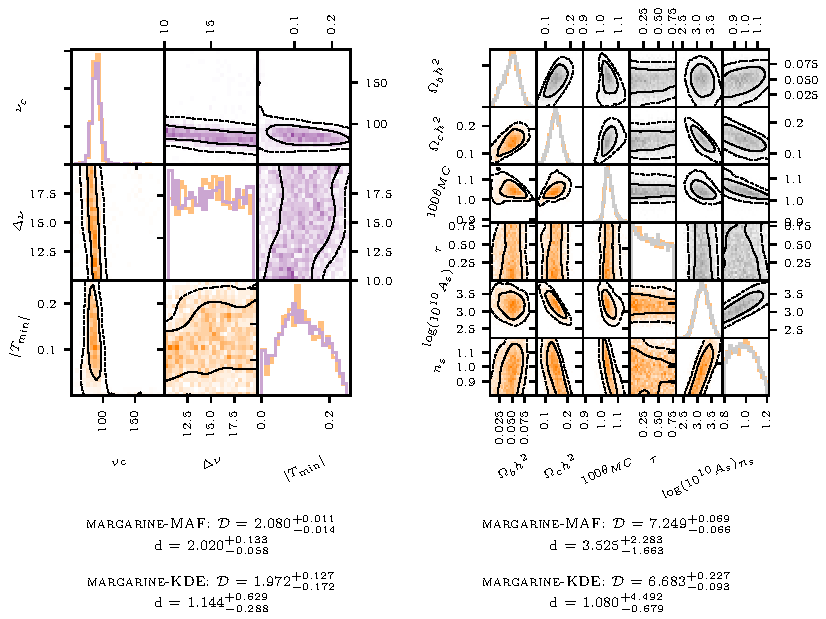
\includegraphics[width=\linewidth]{margarine/figs/cosmo_examples_alt.pdf}
    \caption{\textbf{Left Panel:} The signal subspace, in orange, for a fit to simulated observations of the 21-cm signal with the REACH experiment along with samples, in purple, from KDE trained on the three signal parameters effectively marginalising over the other thirteen parameters in the fit. We report the marginal KL divergence and BMD found for this set of three parameters using both a MAF and KDE. \textbf{Right Panel:} The cosmological subspace for the Year 1 DES samples shown in orange, along with a set of samples taken from a trained MAF in gray. Again, we report the corresponding marginal Bayesian statistics calculated with \textsc{margarine}.}
    \label{fig:cosmo_examples}
\end{figure*}

\subsubsection{Dark Energy Survey}

%The Dark Energy Survey~(DES) is designed to help us understand why the Universe's rate of expansion is accelerating. The goal of the collaboration is to map millions of galaxies, thousands of supernova and large scale cosmic structures in order to help understand the dark energy which makes up 70\% of the universe. The survey has targeted the measurements of the dark matter and dark energy densities as well as the dark energy equation of state~\cite{DES_2005} by investigating galaxy clustering, gravitational lensing and supernova distances.

The Year 1 DES analysis\footnote{We note that the Year 3 DES results have been published~\cite{DES_year3, DES_year3_2021} but that the samples have not been made publicly available.} \cite{Handley_tensions_2019}, as discussed, aimed to constrain the baryon density parameter, $\Omega_b$, the dark matter density parameter, $\Omega_c$, the approximate ratio of the sound horizon to the angular diameter distance, $\theta_{MC}$, the optical depth of the CMB to reionization, $\tau$ and the amplitude and tilt of the power spectrum, $A_s$ and $n_s$. The samples from the cosmological subspace are shown in orange in the right-hand panel of \cref{fig:cosmo_examples}, where we have marginalised over a set of 20 nuisance parameters, along with a MAF reconstruction of the subspace in gray.

Unlike the toy examples and REACH samples, the DES cosmological samples do not have uniform priors and cannot easily be transformed into a space in which the priors are uniform. As a result, we have to use the density estimators built into \textsc{margarine} to evaluate both the log-probability of the posterior and the prior if we want to calculate marginal statistics.

While this is possible, it is expected to lead to an increased uncertainty in the marginal statistics, which can be seen in \cref{fig:cosmo_examples}. In addition, the problem is further complicated by the size of the cosmological parameter space, since we expect larger parameter spaces to be harder to replicate well with \textsc{margarine}, and consequently we expect larger errors on the marginal statistics.

Again the density estimators give us different estimates for the BMD, however the errors are large. From a visual examination of the distribution, we would expect the BMD to be between $\approx3$ and $\approx4$. There is a reasonable agreement between the KL divergence calculated for the cosmological constraints from DES with both the MAF and the KDE. We note that the KL divergence reported here for the DES samples is different from that reported in \cref{fig:joint} but that the two estimates are consistent with each other. The difference stems from the fact that in each analysis we retrained the DES MAF.

\section{Conclusions}
\label{sec:conclusions_margarine}

In this chapter we have demonstrated a number of applications of two different types of density estimator, Masked Autoregressive Flows and Kernel Density Estimators, to the calculation of marginal Bayesian statistics, the efficient modelling of multiple data sets and the derivation and emulation of physical priors. \textsc{margarine} is a multipurpose tool that can be used to enhance our Bayesian analysis workflows.

The evaluation of marginal KL divergences and Bayesian Model Dimensionalities allows for improved comparison of the constraining power of different experiments targeting the same astrophysical or cosmological signals with different systematics or nuisance parameters. In turn, this can lead to improvements in experimental design with techniques that provide more information about the signals of interest being pursued in the future. The calculation of marginal Bayesian statistics has been illustrated in \cite{Scheutwinkel2022b}, \cite{Anstey_lst_2022} and \cref{ch:saras3} \cite{Bevins_saras3_2022}.

The nuisance-free likelihood function allows for more efficient combination of constraints from different data sets, preventing the need to sample instrument specific foreground and systematic effects in joint analysis. This was demonstrated with data from the Planck and Dark Energy Survey experiments, and is explored further with data from the 21-cm power spectrum experiment HERA and sky-averaged 21-cm experiment SARAS3 in \cref{ch:hera_saras3} \citep{Bevins_hera_saras3_2023}.

Finally, \textsc{margarine} can be used to generate non-trivial priors (e.g. \cite{Alsing_bijectors_2021}) either from experimental results or simulations, as illustrated in this chapter. In principle, this allows us to inform the analysis of data from upcoming probes like REACH \citep{de_lera_acedo_reach_2022} or the Simons Observatory \citep{Simons_Obs_2019, Simons_obs_2019b} with results from existing experiments like SARAS3 \citep{Bevins_saras3_2022} and Planck \citep{Planck2018}. We anticipate further development of \textsc{margarine} and additional unexpected applications that evolve as the code is used.
